\begin{titlepage}
    \begin{center}

        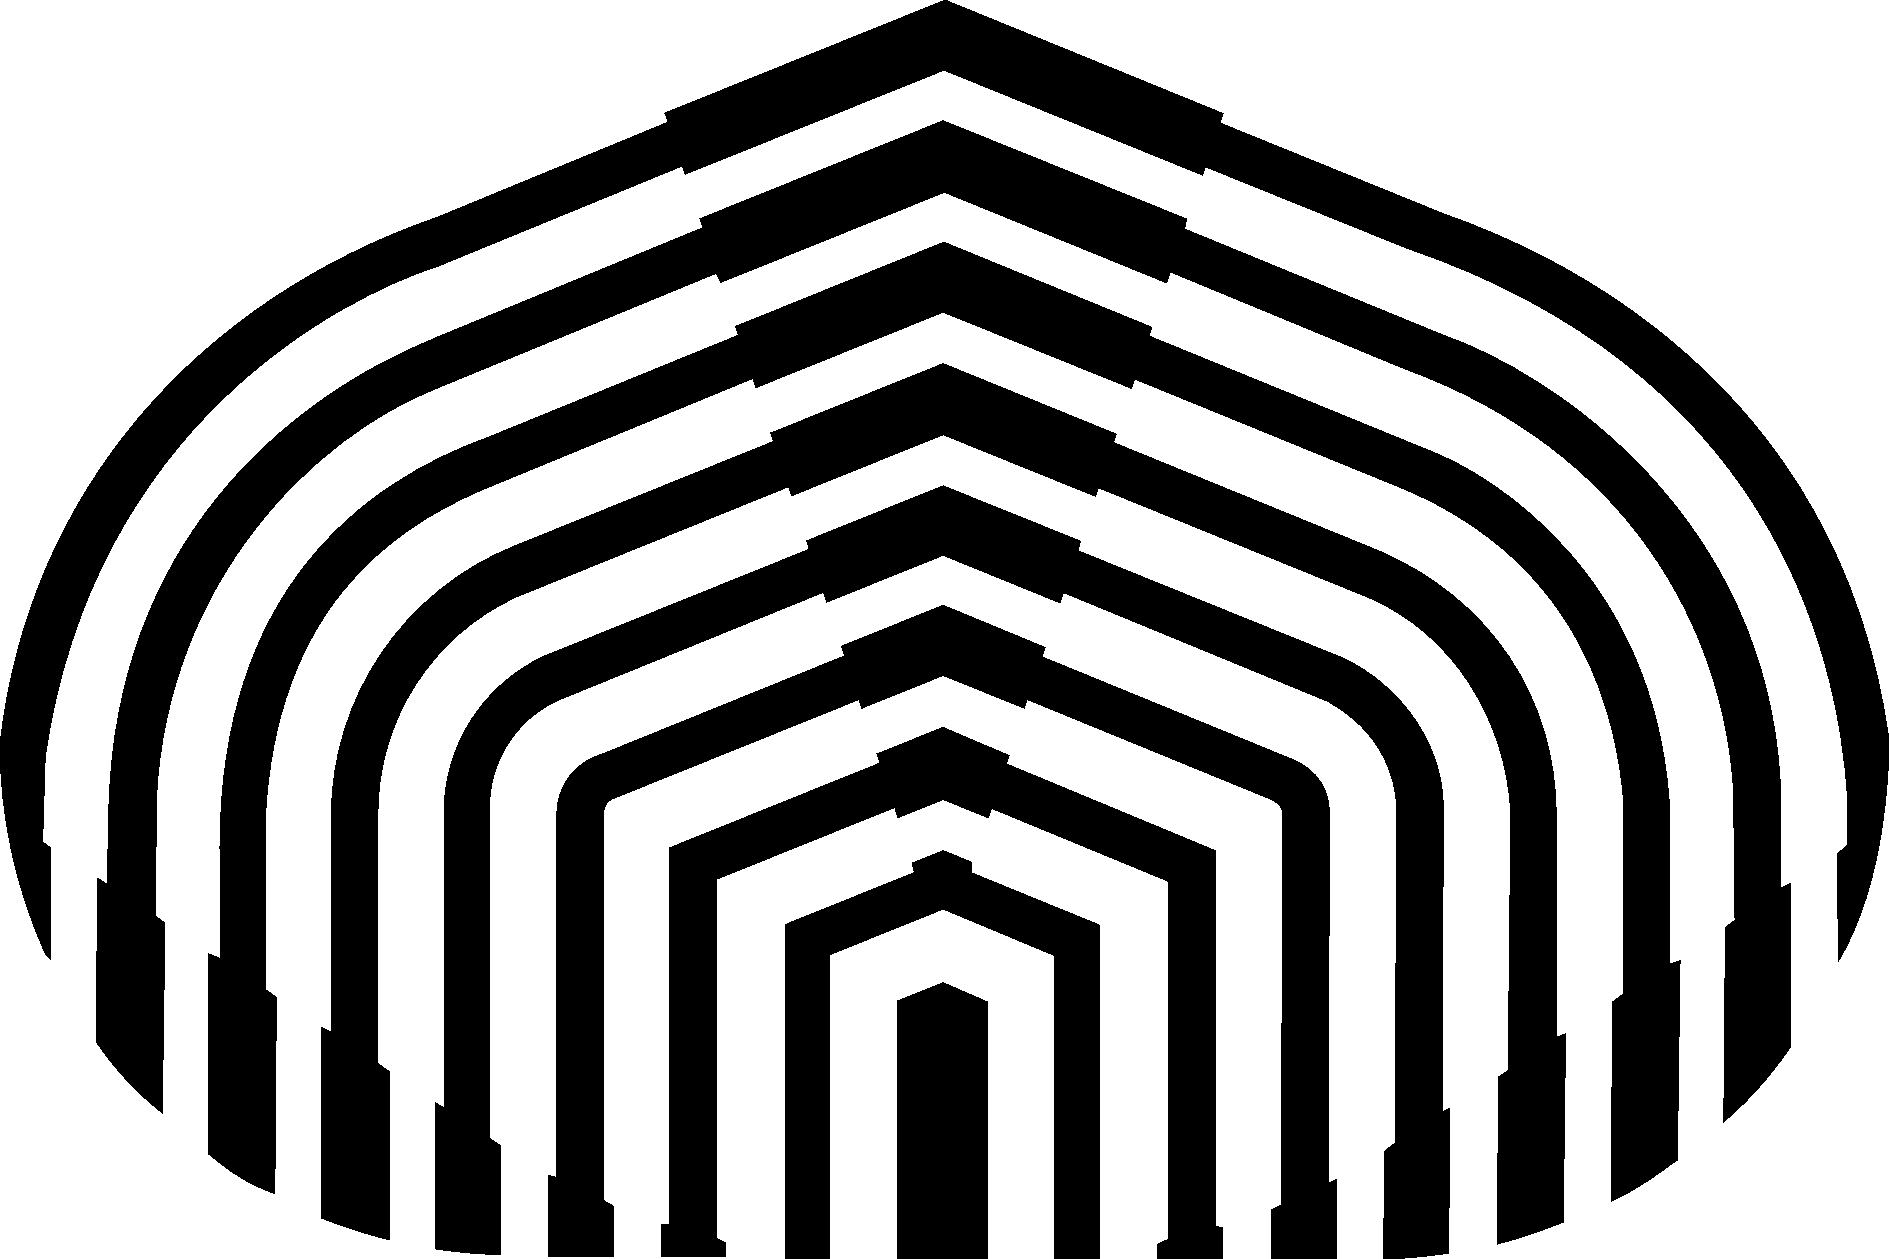
\includegraphics[scale=0.5]{usb.png} \\
        \textsc {\large UNIVERSIDAD SIMÓN BOLÍVAR} \\
        \textsc{DECANATO DE ESTUDIOS PROFESIONALES\\
        COORDINACIÓN DE INGENIERÍA ELECTRÓNICA}\\
        \textbf{SISTEMA DE GENERACIÓN DE MOSAICOS 2D PARA ROBOTS MÓVILES A PARTIR DE VIDEO MONOCULAR} \\
        PROYECTO DE GRADO \\
        PRESENTADO POR: \\
        Victor Yovanni Garcia Carmona, Carnet: 12-10738

    \end{center}
% El resumen debe ser de una sola página
\addtotoc{Resumen}
\abstract
{
    \addtocontents{toc}{\vspace{1em}}
    Al realizar tareas de exploración para el análisis del suelo en espacios aéreos o en fondo marino, es muy común emplear sistemas de adquisición basados en captura de vídeos para su posterior análisis. En la actualidad, el incremento de la tecnología sobre el procesamiento de datos, ha permitido que los algoritmos de visión por computadora coloquen a la cámara como principal sensor para la reconstrucción de entornos recorridos por vehículos móviles. El presente trabajo se encuentra enfocado al análisis e implementación de distintos algoritmos para la reconstrucción de un mosaico 2D (dos dimensiones) del suelo que recorre un robot, a partir de la información proveniente de una cámara monocular ubicada en la parte inferior de este. El robot en cuestión puede realizar recorridos aéreos para realizar la adquisición del vídeo, o incluso trayectorias mas desafiantes como serian las aplicaciones subacuáticas. Para esto, se implementarán distintos algoritmos usando técnicas de procesamiento de imágenes y visión por computadora, para la elaboración de un sistema automatizado que permita generar un mapa en dos dimensiones de la trayectoria recorrida por el vehículo móvil, mejorando la detección de puntos clave y optimizando el calculo de las matrices de transformación para la alineación de imágenes en el mosaico, logrando así un mapa con la menor distorsión posible. Además de realizar análisis sobre el error de proyección de dichas imágenes en el mapa del suelo generado.
    
}

% Las palabras clave son generalmente los nombres de áreas de investigación a
% los cuales está asociado el trabajo. Generalmente son tres o cuatro.
\noindent \begin{small} \textbf{Palabras clave}: mosaico, video monocular, puntos clave, matriz de transformación. 
\end{small}
	
% Iniciar nueva página luego del resumen
\clearpage
\setstretch{1.3}

\end{titlepage}